% !TeX root = skript.tex
\emph{Die nicht-algorithmischen Aspekte dieses Kapitels orientiert sich stark an \cite{barabasi2014network}.}
\bigskip

Eine elementare Aufgabe in Network Science ist es die Wichtigkeit von Knoten zu bewerten --- man spricht auch \aside{Zentralität: Wichtigkeit eines Knotens} von der \emph{Zentralität} der Knoten.
Die Anzahl der Nachbarn (Grad, engl. degree) ist eine sehr einfache Metrik mit direkter Intuition:
wenn ein Knoten überdurchschnittlich viele Nachbarn hat, dann steht die Vermutung im Raum, dass diesem Knoten auch eine überdurchschnittlich wichtige Funktion im Netzwerk zu kommt.
Daher wollen wir die Verteilung von Graden in Graphen in diesem Kapitel genauer betrachten.

Zur Wiederholung:
In einem ungerichteten Graphen~$G=(V,E)$ beschreibt
\begin{align}
    \deg(u) = \card{\twoset{e}{e \in E\text{, \sd\,} u \in e}}
\end{align}
die Anzahl der Nachbarn von Knoten~$u$.
Die \aside{Grad\underline{sequenz}} Gradsequenz~$\degseq_G$ (falls $G$ klar ist auch nur $\degseq$) von $G=(V,E)$ mit $V=\set{v_1, \ldots, v_n}$ ist dann einfach die Auflistung aller Grade im Graphen
\begin{align}
    \degseq_G = (\deg(v_1), \deg(v_2), \ldots, \deg(v_n)).
\end{align}
Beobachte, dass für jede $\degseq_G$ von $G=(V,E)$ gilt:
\begin{align}
    \sum_{v \in V} \deg(v) = 2 \card{E}
\end{align}


\section{Knotengrade in $\Gnp$}
\begin{figure}
    \begin{center}
        \includegraphics[width=0.6\textwidth]{data/gnp_degrees.pdf}
    \end{center}
    \caption{
        Histogramm der Gradsequenz~$\degseq_G$ eines Graphen~$G \sim \Gnp$.
        Die vertikale Linie zeigt den Durchschnittsgrad $\bar k$,
        die Punkte die Vorhersage mittels Binomialverteilung.
    }
    \label{fig:histogram_grade_gnp}
\end{figure}

Die Gradsequenz~$\degseq_G$ ist ein konkreter \qq{Messwert} für einen Graph~$G$.
Für die meisten Graphen mit vielen Knoten können wir --vereinfachend-- davon ausgehen, dass die einzelnen Grade unabhängig aus einer Wahrscheinlichkeitsverteilung gezogen wurden.
Wir \aside{Grad\underline{verteilung}} nennen diese Wahrscheinlichkeitsverteilung dann die \emph{Gradverteilung}.
Das ist besonders sinnvoll, wenn $G$ selbst aus einem Zufallsgraph stammt.
Dann versuchen wir die Gradverteilung auf das durch den Zufallsgraphen definierte Ensemble auszuweiten.
Im Folgenden betrachten wir etwa die Gradverteilung von $\Gnp$ Graphen.

Aus \cref{subsec:anzahl_kanten_in_gnp} wissen wir bereits, dass die Kantenanzahl eines $\Gnp$ Graphen binomial verteilt ist.
Die Analyse für Grade läuft analog, allerdings nicht für $\binom n 2$ Einträge der Adjazenzmatrix, sondern nur für $n-1$ (da Eigenschleifen verboten sind: $-1$).
Der Grad~$\deg(u)$ eines Knotens~$u$ ist also ebenfalls binomial verteilt:
\begin{align}
    \prob{\deg(u) = k} =
    \underbrace{\binom{n-1}{k}}_\text{\begin{minipage}{9em}\centering Anzahl an möglichen\\[-0.5em] Nachbarschaften\end{minipage}}
    \ \cdot \
    \underbrace{p^k}_\text{Existenz der $k$ Kanten}
    \ \cdot \
    \underbrace{(1-p)^{n-1-k}}_\text{\begin{minipage}{10em}\centering Abwesenheit der \\[-0.5em] restlichen Kanten\end{minipage}}
    \label{eq:gradverteilung_gnp}
\end{align}
Daher gilt also $\expv{\deg(u)} = (n-1)p$.

Wie in \cref{fig:histogram_grade_gnp} dargestellt, approximiert eine konkrete Gradsequenz~$\degseq_G$ die Gradverteilung schon sehr gut.
Der Erwartungswert sollte daher gegen den Durchschnittsgrad $\bar d = 2m / n$ konvergieren, \dh $\expv{\deg(u)} \approx \bar d$.
Dann gilt also:
\begin{align}
    \bar d \approx \expv{\deg(u)} & = (n-1)p \\
    p \approx \frac{\bar d}{n-1} \label{eq:gnp_p_von_avg_deg}
\end{align}

Für tiefere analytische Untersuchen ist die Binomialverteilung ein bisschen unhandlich.
Wir wollen daher eine Approximation (siehe \cite{barabasi2014network}) für dünne Netzwerke finden.
Aus $m = \Oh{n \log n}$ folgt direkt $\bar d = \Oh{\log n}$.
Somit ist also $\bar d \ll n$ eine gute Annahme für dünne Graphen.

\medskip

Betrachten wir also zunächst den Binomialkoeffizienten in \cref{eq:gradverteilung_gnp}:
\begin{align}
    \binom{n-1}{k}
     & = \frac{1}{k!} \cdot \frac{(n-1)!}{(n-1-k)!}                                                              \\
     & = \frac{1}{k!} \cdot \left[ (n-1) \cdot (n-1-1) \cdot (n-1-2) \cdot \ldots \cdot (n-1-(k - 1))    \right] \\
     & \approx \frac{1}{k!} \left[ n- 1 \right]^k
\end{align}

Im letzten Schritt nutzten wir aus, dass $k \ll n$ und somit $n-1 \approx n-k$.
Die Wahrscheinlichkeit, in \cref{eq:gradverteilung_gnp}, dass $n-1-k$ Nachbarn \emph{nicht} existieren, können wir wie folgt auffassen:
\begin{align}
    (1 - p)^{n-1-k} & = \exp\left[ \ln\left((1 - p)^{n-1-k}  \right) \right]
\end{align}

\noindent
Konzentrieren wir uns nun zunächst auf den Logarithmus:
\begin{align}
    \ln\left((1 - p)^{n-1-k}  \right)  =
    (n-1-k) \ln (1 - p)
    \approx - (n-1-k) p
\end{align}

\noindent
Im letzten Schritt nutzen wir die Abschätzung $\ln(1+x) \approx x$, welche für kleine $x \ll 1$ aus der Taylorreihe von $\ln(1+x) = x - \Oh{x^2}$ resultiert.
Nun können wir \cref{eq:gnp_p_von_avg_deg} nutzen, um $p$ zu substituieren:
\begin{align}
    - (n-1-k) p \approx - (n-1-k) \frac{\bar d}{n-1} \approx - \bar d
\end{align}

\noindent
Somit folgt letztendlich:
\begin{align}
    (1 - p)^{n-1-k} = \exp\left[ \ln\left((1 - p)^{n-1-k}  \right) \right] \approx \exp(-\bar d)
\end{align}

\noindent
Damit haben wir nun alle Bausteine, um die Binomialverteilung zu approximieren:
\begin{align}
    \prob{\deg(u) = k}
     & = \textcolor{red}{\binom{n-1}{k}} \cdot p^k \cdot \textcolor{blue}{(1-p)^{n-1-k}}                       \\
     & \approx \textcolor{red}{\frac{1}{k!} \left[ n- 1 \right]^k} p^k \textcolor{blue}{\exp(-\bar d)}         \\
     & \stackrel{(\ref{eq:gnp_p_von_avg_deg})}{\approx}
    \textcolor{red}{\frac{1}{k!} \left[ n- 1 \right]^k} [\frac{\bar d}{n-1}]^k \textcolor{blue}{\exp(-\bar d)} \\
     & = \frac{\bar d^k}{k!} \exp(-\bar d)
\end{align}

\noindent
Beim letzten Ausdruck handelt es sich um die Poissonverteilung:

\begin{definition}
    Für \aside{Poissonverteilung} $\lambda > 0$ ist die ganzzahlige und nicht-negative Zufallsvariable $X$ \emph{poisson-verteilt}, falls
    \begin{align}
        \prob{X = k} = \frac{\lambda ^k}{k!} \exp(-\lambda)
    \end{align}

    Dann gilt, dass der Erwartungswert $\expv{X} = \lambda$ und die Varianz $\var(X) = \lambda$ identisch sind.
\end{definition}

\begin{figure}
    \begin{center}
        \includegraphics[width=0.5\textwidth]{data/binom_vs_poisson.pdf}
    \end{center}
    \caption{
        Vergleich von Binomialverteilung und Poissonverteilung für fixierten Durchschnittsgrad $\bar k = 100$.
        Je größer $n$, desto eher ist die Approximations-Voraussetzung $\bar k \ll n$ erfüllt, und desto mehr sind Binomialverteilung und Poissonverteilung deckungsgleich.
    }
    \label{fig:binom_vs_poisson}
\end{figure}

\bigskip

Aus dieser Approximation mittels Poissonverteilung ergibt sich eine interessante Einsicht.
Während \aside{Für $\bar k \ll n$ ist die Gradverteilung nur von $\bar k$ abhängig} die Binomialverteilung von der Knotenanzahl~$n$ und Kantenwahrscheinlichkeit~$p$ abhängt, hat die Poissonverteilung nur den Parameter~$\lambda = p / (n-1) \approx \bar k$.
Die Interpretation hiervon ist, dass für $\bar k \ll n$ die Gradverteilung nur vom Durchschnittsgrad~$\bar k$, nicht aber von der Knotenanzahl im Graphen abhängen sollte.
\Cref{fig:binom_vs_poisson} untermauert diese Interpretation:
Die Binomialverteilungen der zwei größten Netze sind mit dem bloßen Auge nicht mehr von der Poissonverteilung unterscheidbar.

Diese Einsicht können wir uns wie folgt erklären:
Die Poissonverteilung beschreibt die Anzahl von Ereignissen, die innerhalb eines fixierten Intervalls auftreten, wenn die mittlere Rate konstant ist.
In diesem Bild ist jede Zeile der Adjazenzmatrix solch ein Intervall und die mittlere Rate entspricht der durchschnittlichen Anzahl an Einsen pro Zeile --- also dem Durchschnittsgrad~$\bar d$.

Beachte auch, dass die Varianz der Poissonverteilung mit $\var(X) = \bar d$ größer ist als die Varianz der Binomialverteilung $\var(X) = n p(1 - p) \approx \bar d (1 - \bar d / n )$, wobei der geklammerte Faktor kleiner als $1$ ist.

\section{Power-Law Gradverteilung}
\begin{figure}
    \begin{center}
        \includegraphics[width=\textwidth]{data/dblp_degree_distribution.pdf}
    \end{center}
    \caption{Gradverteilung von zwei beobachteten Netzwerken~\cite{Penschuck_2020} verglichen mit drei analytischen Verteilungen.}
    \label{fig:grade_in_dblp}
\end{figure}

In \cref{fig:grade_in_dblp} stellen wir die Gradverteilung, genauer das Histogramm der Gradsequenz, von zwei beobachteten Netzwerken dar.
Die genaue Herkunft der Graphen ist hier nicht wichtig; viele beobachte komplexe Netzwerke zeigen einen qualitativ ähnlichen Verlauf.
Was sofort auffällt, ist, dass die rot dargestellte Binomialverteilung keine satisfaktionsfähige Übereinstimmung mit der beobachteten Verteilung zeigt:

\begin{itemize}
    \item Die  Binomialverteilung sagt vorher, dass die meisten Knoten grob den Durchschnittsgrad haben müssten.
          Zu beiden Richtungen ---sprich für kleinere und größere Grade--- sollte es deutlich weniger Knoten geben.

    \item Der \aside{Binomialverteilung / Poissonverteilung haben keine extremen Gerade} maximale Grad ($\approx 30$ im linken Schaubild) sollte in etwa dieselbe Größenordnung haben, wie der Durchschnittsgrad ($\approx 10$).
\end{itemize}

\noindent
Das beobachtete Netzwerk hat jedoch ein signifikant anderes Verhalten:
\begin{itemize}
    \item Die meisten Knoten haben sehr geringen Grad --- deutlich geringer als der Durchschnittsgrad.
    \item Der maximal Grad ($\approx 4000$) ist viel höher als der Durchschnittsgrad ($\approx 10$).
          Offensichtlich \qq{ziehen} diese wenigen Knoten den Durchschnittsgrad also maßgeblich nach oben.
          Es sollte daher auch nicht überraschend, dass diese sog. Hubs viele Eigenschaften des Netzwerks prägen.
\end{itemize}

In \cref{fig:grade_in_dblp} \aside{Power Law entspricht einer Geraden im Histogramm} fällt ebenfalls auf, dass sich das Histogramm durch eine Gerade (im Folgenden als Linie bezeichnet um Verwechselung mit Grad auszuschließen) relativ gut approximieren lässt.
Dies trifft besonders auf größere Grade zu --- aufgrund des doppel-logarithmischen Plots stellen diese in absoluten Zahlen einen deutlich größeren Bereich dar, als die Abbildung suggeriert.
Wir können also als Arbeitshypothese annehmen, dass die meisten Knotengrade gut durch eine Linie im log-log-Plot beschrieben werden.
Welche Gesetzmäßigkeit können wir daraus ableiten?

Wir können eine Linie mittels $y = mx + b$ beschreiben.
Im log-log-Plot sind nun beide Achsen skaliert.
Es gilt daher $x = \log d$ und $y = \log h(d)$, wobei $d$ der Grad sei und $h(d)$ die Häufigkeit widerspiegele.
Dann gilt:
\begin{align}
    y               & = mx + b              \\
    \log h(d)       & = m\log d + b         \\
    \exp[\log h(d)] & = \exp[\log(d^m) + b] \\
    h(d)            & = \exp(b) \cdot d^m
\end{align}

Die Häufigkeit skaliert also proportional zu $d^m$.
Wir \aside{Potenzgesetz, Power Law: $p \propto d^{-\gamma}$ für (meist) $2 < \gamma < 3$} sprechen daher von einem Potenzgesetz (engl. Power Law).
Da die Anzahl der Beobachtungen für größere Grade abnimmt, ist der Exponent immer negativ.
Wir schreiben ihn daher als $d^{-\gamma}$, wobei der sog \emph{Power Law Exponent}~$\gamma$ aus dem Intervall $2 < \gamma < 3$ stammt (falls nicht anders angegeben).

Um eine Wahrscheinlichkeitsverteilung $p(d)$ zu erhalten, müssen wir die Terme noch skalieren:
\begin{align}
    p(d) = C' h(d) = \underbrace{C'\exp(b)}_{:= C} d^{-\gamma}
\end{align}

\noindent
Wir absorbieren also den $\exp(b)$ Faktor in die Normierungskonstante~$C$:
\begin{align}
    1                & \stackrel{!}{=} \sum_{i=1}^\infty C d^{-\gamma}                          \\
    C                & = \frac{1}{\sum_{i=1}^\infty d^{-\gamma}}      = \frac{1}{\zeta(\gamma)} \\
    \nonumber                                                                                   \\
    \Rightarrow p(d) & = \frac{d^{-\gamma}}{\zeta(\gamma)}
\end{align}

Die Funktion $\zeta(\gamma)$ ist die sog. Riemann-Zeta-Funktion (wir werden diese im Folgenden nicht dediziert betrachten).

Beobachte, dass $0^a$ für $a < 0$ eine Division durch $0$ darstellt.
Daher ist $p(0)$ nicht definiert und wird explizit in der vorherigen Summierung herausgenommen.
Sollte ein Graph $n_0>0$ isolierte Knoten beinhalten, betrachtet man diese idR als Sonderfall.
Wir definieren also $p(0) = n_0 / n$ und skalieren die Power Law Verteilung auf $1  - n_0 /n$.

\def\dmin{\ensuremath{{d_{\text{min}}}}}
\def\dmax{\ensuremath{{d_{\text{max}}}}}
\def\dnc{\ensuremath{{d_{\text{nc}}}}}

Umgekehrt ist es oft auch sinnvoll, die minimalen und maximalen Grade $\dmin < \dmax$ explizit zu beschränken.
Wir müssen dann nur die Skalierungskonstante auf den kleineren Bereich anpassen:
\begin{align}
    C_{\dmin,\dmax} = 1 / \sum_{d = \dmin}^\dmax d^{-\gamma}
\end{align}

\begin{exercise}\label{aufg:dmin_dmax}
    Entwickele durch ein paar stichprobenartige Rechnungen eine Intuition, welchen Einfluss $\dmin$ und $\dmax$ auf $C_{\dmin,\dmax}$ haben.
    Erkläre deine Beobachtungen.
\end{exercise}

\subsection{Kontinuierlicher Formalismus}
In der Herleitung des diskreten Power Law haben wir bereits in der Normierung die transzendente $\zeta(\gamma)$ Funktion gesehen.
Weitere Analysen werden durch die diskrete Natur der Verteilung nicht einfacher.
Daher ist es oft bequemer die Gradverteilung als kontinuierliches Konstrukt anzunehmen.
An der Grundform ändert sich dann erst einmal nichts, außer, dass der Grad nun eine strikt positive reelle Zahl sein darf:

\begin{align}
    p(d) = C d^{-\gamma} \quad\quad d \in \mathbb R_{> 0}
\end{align}

Für die Normierung steht uns nun aber das Integral statt der Summe zur Verfügung und führt zu deutlich handlicheren Ergebnissen.
Allerdings reicht es nicht mehr, nur $d = 0$ auszuschließen.
Wir definieren die Verteilung daher immer für einen expliziten minimalen Grad~\dmin; \dmax{} lässt sich analog einführen, wir verzichten aber darauf (siehe auch \cref{aufg:dmin_dmax}).

\begin{align}
    C_\dmin                           & = 1 / \int_{d=\dmin}^\infty d^{-\gamma} \intd k                                                \\
                                      & = 1 / \left[ \frac{1}{-\gamma + 1} d^{-\gamma + 1}  \right]_\dmin^\infty                       \\
                                      & = 1 / \left( - \frac{1}{-\gamma + 1} \dmin^{\textcolor{red}{1 - \gamma}}  \right)              \\
                                      & = \underbrace{( \gamma-1)}_{\text{$> 0$ für $\gamma > 1$}} \dmin^{\textcolor{red}{\gamma - 1}} \\
    \nonumber                                                                                                                          \\
    \Rightarrow\quad p_\text{cont}(d) & = (\gamma-1) \dmin^{\gamma - 1} \cdot d^{-\gamma}
\end{align}

Wichtig ist nun allerdings, dass $p_\text{cont}(d)$ keine natürliche punktweise Interpretation mehr hat.
Vielmehr müssen wir nun immer die Wahrscheinlichkeit, dass ein $X$ aus einem Intervall $[a, b]$ stammt, betrachten:
\begin{align}
    \prob{a \le X \le b} = \int_{a}^b p_\text{cont}(d) \intd k
\end{align}

\begin{exercise}
    Berechne den Erwartungswert der kontinuierlichen Power Law Verteilung mit fixierten Grenzen $0 < \dmin < \dmax \le \infty$.
\end{exercise}

\subsection{Größe von Hubs}\label{subsec:groesse_von_hubs}
Eine zentrale Motivation von Poissonverteilungen abzurücken, war es, dass sie keine außergewöhnlich großen Grade zulassen.
Daher wollen wir den größten Grad eines Knotens in einer Power Law Verteilungen abschätzen.

Konkret suchen wir die Größe \dnc{} (engl. natural cut-off), sodass wir nur einen Knoten mit Grad $\ge \dnc$ erwarten.
Es muss also gelten, dass $\prob{\deg(u) \ge \dnc} = 1 / n$ ist:
\begin{align}
    1/n                                & = \int_\dnc^\infty p(d) \intd d                                                               \\
                                       & = C \int_\dnc^\infty d^{-\gamma} \intd d                                                      \\
                                       & = (\gamma-1) \dmin^{\gamma - 1} \left[ \frac{d^{-\gamma + 1}}{-\gamma +1} \right]_\dnc^\infty \\
                                       & = (\gamma-1) \dmin^{\gamma - 1} \left( 0 - \frac{\dnc^{-\gamma + 1}}{-\gamma +1} \right)      \\
                                       & = \dmin^{\gamma - 1} \dnc^{1 - \gamma}                                                        \\
    \nonumber                                                                                                                          \\
    \Rightarrow\quad \dnc^{\gamma - 1} & = \dmin^{\gamma - 1} n                                                                        \\
    \Leftrightarrow\quad \dnc          & = \dmin n^{1/(\gamma - 1)}
\end{align}

Für $\gamma  < 2$ sagt diese Gleichung einen Knoten voraus, der mehr Nachbarn hat, als es Knoten im Graphen gibt.
Dies ist nur eines von vielen Indizien, die zu unserer Annahme $\gamma > 2$ führen.
Für $\gamma \searrow 2$ (\dh rechts-seitiger Grenzwert für $\gamma \to 2$) skaliert der maximale Grad als $\Theta(n)$.
Für $\gamma = 3$ ist er noch $\Theta(\sqrt{n})$ et cetera.

\section{Wie entstehen eine Power Law Gradverteilungen?}
Das Entstehen von Power Law Verteilungen in  unterschiedlichsten Netzwerken gibt Anlass zu der Frage, wie solche Verteilungen denn eigentlich entstehen.
Barab{\'{a}}si und Albert~\cite{barabasi1999emergence} geben eine sehr populäre Erklärung, die besonders durch ihre Simplizität besticht.
Ähnliche Techniken wurden jedoch bereits früher verfolgt (\zB~\cite{10.2307/1716232}).

Die beiden Autoren schlagen neues Modell vor, das wir im Folgenden BA-Modell nennen.
Es stellt zwei implizite Annahmen von \Gnp und \Gnm Graphen infrage:
\begin{itemize}
    \item
          In \Gnp Graphen fixieren wir die Knotenanzahl initial und ändern diese dann nicht mehr.
          Netzwerke in der freien Wildbahn unterliegen jedoch in der Regel einer Dynamik:
          Knoten und Kanten kommen hinzu und verschwinden ggf. wieder.

    \item
          Wenn wir einen Knoten im \Gnp Graphen als Spieler interpretieren, nimmt das Modell an, dass die Nachbarn rein zufällig ausgesucht werden.
          Tatsächlich unterliegen aber viele Handlungen im echten Leben einem sog. Bias (\dh einer verzerrten Wahrscheinlichkeitsverteilung).

          Dies ist besonders auffällig, wenn es zu einer Form von Selektion kommt.
          So kann kein Mensch alle Webseiten kennen (und dann darauf verlinken); von Facebook, Twitter, und Google haben die Meisten aber gehört.
          Wenn also eine zufällige Person einen Artikel schreibt, ist es deutlich wahrscheinlicher, dass ein Link zu Twitter entsteht, als ein Link zu einer bestimmten obskuren Webseite.
\end{itemize}

\subsection{Das BA Modell}
Das \aside{BA Modell beinhaltet Wachstum und Preferential Attachment} BA-Modell trägt beiden Beobachtungen Rechnungen.
Wir starten zunächst mit einem (meist) kleinen und zusammenhängenden Startgraphen mit $n_0$ Knoten und $m_0$ Kanten.
Dann fügen wir iterativ $N$ neue Knoten hinzu und erhalten so am Ende $n = n_0 + N$ Knoten.
Jeder neue Knoten verbindet sich mit $\nu \le n_0$ zufällig gewählten Nachbarn.
Wir sagen, dass der $t$-te neue Knoten im $t$-ten Zeitschritt (für $t = 1,2, \ldots, N$) hinzufügt wird;
unmittelbar nach dem $t$-ten Zeitschritt hat der Graph also
\begin{align}
    n_t = n_0 + t \text{ Knoten} \quad \text{und} \quad
    m_t = m_0 + \nu t \text{ Kanten}.
\end{align}
Analog bezeichnen wir den Grad von Knoten $v$ nach Zeitschritt $t$ als $\deg_t(v)$.
Für $t \ggg n_0$ konvergiert das BA Modell also gegen einen Durchschnittsgrad von
\begin{align}
    \bar{d_t} = \frac{1}{n_t} \sum_{v} \deg_t(v) = 2 \frac{m_0 + \nu t}{n_0 + t} \to 2 \nu
\end{align}

Um den zuvor genannten Bias zu implementieren, nehmen wir aber an, dass Knoten mit vielen Nachbarn besonders bekannt sind und unterstellen einen linearen Zusammenhang.
Wenn wir also aus zwei Knoten $a$ und $b$ mit $\deg(a) = 2\deg(b)$ wählen müssen, ziehen wir Knoten~$a$ mit doppelter Wahrscheinlichkeit.
Sei $p_t(v)$ die Wahrscheinlichkeit, dass wir Knoten $v$ in Zeitschritt $t + 1$ ziehen.
Dann gilt:
\begin{align}
    p_t(v) = \frac{\deg_t(v)}{\sum_u  \deg_t(u)} = \frac{\deg_t(v)}{2(m_0 + \nu t)}
\end{align}

\subsection{Dynamik in der Gradverteilung}
Der beschriebene Bias wird \emph{Preferential Attachment} bezeichnet.
Es bildet sich eine positive Rückkopplung:
ein Knoten mit hohem Grad wird wahrscheinlicher als andere Knoten gezogen.
Ein gut vernetzter Knoten akkumuliert also schneller neue Nachbarn, und wird dadurch noch berühmter.
Der Prozess liegt daher einigen Sprichworten zugrunde, \zB \qq{the rich get richer} (dt. \qq{Der Teufel ... auf den größten Haufen}).
Es gibt diverse Methoden zur formalen Analyse des Prozess --- eine der einfachsten ist der kontinuierliche Formalismus, in der wir Knotengrade und die Zeit durch reelle Zahlen approximieren.
Der Einfachheit halber, verwenden wir dennoch weiterhin den Begriff Zeitschritt, womit wir ein Zeitintervall von Einheitslänge meinen.

Wir gehen davon aus, dass die $\nu$ Kanten in einem Zeitschritt gleichzeitig gezogen werden;
es können also Mehrfachkanten entstehen.
Die erwartete Anzahl an Nachbarn, die Knoten~$v$ in einem Schritt~$t+1$ ansammelt, ist dann also $\nu p_t(v)$.
Da die Zeit ab jetzt kontinuierlich angenommen wird, \emph{fixieren wir einen Knoten $v_i$}, der zum Zeitpunkt $t_i$ hinzugefügt wird, und betrachten seinen Grad als zeitabhängige Funktion $d(t)$.
Es gilt $d(t) = 0$ für $t < t_i$ und $d(t_i) = \nu$.\footnote{
    Wir weichen an dieser Stelle von der diskreten Notation ab, bei der erst $d(t_i + 1) = \nu$ wäre.
    Dies hat aber keinen signifikanten Einfluss auf unsere Analyse und vereinfacht die Formeln.
}
Analog sei $m(t) = m_0 + \nu t$ die kontinuierliche Kantenanzahl.

Das Wachstum $\intd d(t) / \intd t$ der Funktion hängt nun vom Grad $d(t)$ selbst ab.
Es ergibt sich somit die folgende Differentialgleichung:
\begin{align}
    \frac{\intd d(t)}{\intd t}
     & = \nu p_t(v)
    = \nu \frac{d(t)}{2 m(t)}
    = \nu \frac{d(t)}{2(m_0 + \nu t)}                                         \\
     & \stackrel{t \gg 0}{\approx} \nu \frac{d(t)}{2 \nu t} = \frac{d(t)}{2t}
\end{align}

Diese spezielle Differentialgleichung lässt sich relativ einfach lösen.
Wir teilen beide Seiten durch $d(t)$ (ab Zeitpunkt $t \ge t_i$ gilt $d(t) > 0$) und integrieren dann von $t_i$ (dem Zeitpunkt zu dem der Knoten $v_i$ hinzugefügt wurde) bis $T$:

\begin{align}
    \int_{t_i}^T  \frac{\frac{\intd d(t)}{\intd t}}{d(t)} \intd t & = \int_{t_i}^T \frac{1}{2t} \intd
\end{align}

\noindent
Die rechte Seite ist ein Standardintegral:
\begin{align}
    \int_{t_i}^T \frac{1}{2t} \intd = \left[ \frac 1 2 \log t \right]_{t_i}^T = \frac 1 2 \log\left(\frac{T}{t_i}\right)
\end{align}

Die linke Seite lässt sich mittels Substitution von $u = d(t)$ und $\intd u = \frac{\intd d(t)}{\intd t} \intd t$ analog zur rechten Seite integrieren.
Somit folgt insg:
\begin{align}
    \log\left(\frac{d(T)}{d(t_i)}\right) & = \frac 1 2 \log \left(\frac{T}{t_0}\right)                             \\
    \frac{d(T)}{d(t_i)}                  & = \sqrt{\frac{T}{t_i}}                                                  \\
    d(T)                                 & = d(t_i) \sqrt{\frac{T}{t_i}} = \nu \left( \frac{T}{t_i} \right)^\beta,
\end{align}
wobei $\beta = 1/2$ der \aside{Dynamischer Exponent $\beta = 1/2$} dynamische Exponent bezeichnet wird.

Diese unscheinbare Gleichung gibt bereits viel über das Verhalten von BA Netzwerken preis.
Zunächst fällt auf, dass der Grad monoton wächst (es gibt schließlich keinen Prozess, um ihn zu reduzieren).
Die erwartete Anzahl der Nachbarn von verschiedenen Knoten $v_i$ und $v_j$ unterscheidet sich zudem nur durch die Zeitpunkte $t_i$ und $t_j$ zu denen sie hinzugefügt wurden.
Je früher ein Knoten ins Netz eintrat, desto höher ist sein erwarteter Grad --- der sogenannte \aside{first-mover advantage} \emph{first-mover advantage}.

Die Situation für später hinzugekommen ist sogar noch schlechter, als man zunächst erwarten würde:
Die Startzeit~$t_i$ skaliert mit $\sqrt{1 / t_i}$ in den Knotengrad.
Während ein frühes Mitglied innerhalb einer gewissen Zeitspanne nach ihrem Beitritt noch $X$ Nachbarn anhäufen konnte, bekommt ein späterer Knoten in derselben Zeit nur noch einen Bruchteil dieser Knoten.
Dies liegt einfach daran, dass es in späteren Zeitpunkten mehr \qq{Konkurrenz} gibt und somit Nachzügler kaum Aufmerksamkeit bekommen.
Dies kann man als Schwäche des Netzwerks interpretieren, da die einzige Chance im Mittel erfolgreich zu sein darin besteht, früh beigetreten zu sein.

\subsection{Gradverteilung des BA-Modells}
Im vorherigen Kapitel haben wir herausgefunden, dass der Grad eines Knotens~$v_i$ nach dem Beitritt ins Netz zu Zeitpunkt $t_i$ gemäß $d(t) = \nu (t  / t_i)^{1/2}$ wächst.
Wir müssen dieses Ergebnis noch in eine Gradverteilung zum Zeitpunkt $T \ggg 1$ übersetzen.

Die Intuition hierfür ist folgende:
Wir wissen, dass wir zum Zeitpunkt~$T$ insgesamt $T$ zufällige Knoten hinzugefügt haben und können annehmen, dass wir das in einem regelmäßigen Takt getan haben.
Dann müssen wir nur noch extrapolieren, welchen Grad wir für jeden diesen Knoten zu Zeitpunkt $T$ erwarten.
Konkret fragen wir uns, wann ein Knoten eingefügt werden musste, \sd er höchsten Grad $k$ hat:
\begin{align}
                    &  & d(T)                                   & < k         \\
    \Leftrightarrow &  & \nu \left(\frac{T}{t_i}\right)^\beta   & < k         \\
    \Leftrightarrow &  & \frac{\nu}{k} T^\beta                  & < t_i^\beta \\
    \Leftrightarrow &  & \left(\frac{\nu}{k}\right)^{1/\beta} T & < t_i
\end{align}

Wir erwarten also, dass Knoten, die ab dem Zeitpunkt $t_i > (\nu / k)^{1/\beta} T$ eingefügt wurden, einen Grad von höchsten $k$ haben.
Davon gibt es $T - (\nu / k)^{1/\beta} T$ viele!
Sei $X$ nun ein zum Zeitpunkt~$T$ uniform gewählter Knoten und $P(k) = \prob{X \le k}$ die kumulative Verteilungsfunktion.
Dann gilt:
\begin{align}
    P(k) & = \prob{X \le k} = \frac{T - (\nu / k)^{1/\beta} T}{n_T} = \frac{T - (\nu / k)^{1/\beta} T}{n_0 + T} \\
         & \stackrel{T \gg n_0}{\approx} \frac{T - (\nu / k)^{1/\beta} T}{T} = 1 - (\nu / k)^{1/\beta}
\end{align}

Für die Gradverteilung benötigen wir nun die Wahrscheinlichkeitsverteilung $p(k)$; also die Ableitung von $P(k)$:
\begin{align}
    p(k) & = \frac{\intd P(k)}{\intd k} = \frac{\intd}{\intd k} (1 - (\nu / k)^{1/\beta}) \\
         & = - \nu ^ {1/\beta}  \frac{\intd}{\intd k} k ^{-1/\beta}                       \\
         & = \frac{1}{\beta} \nu ^{1 / \beta} k^{-\beta - 1}                              \\
         & = 2 \nu^2 k^{-3}
\end{align}

Hierbei sind $2 \nu^2$ konstante Vorfaktoren.
Durch Parametervergleich ergibt sich also eine Power Law Verteilung mit Exponent $\gamma = 3$.

\section{Generieren von BA Graphen}
\begin{algorithm}[t]
    \KwIn{Startgraph als Kantenliste $E_0$ über Knoten $1, \ldots, n_0$. Anzahl der Zufallsknoten~$N$ sowie deren Nachbaranzahl~$\nu$.}
    \KwOut{Kantenliste $E$}
    \SetKwFunction{pushback}{pushBack}

    Allokiere leeres Array $E$ mit Kapazität $2(|E_0| + \nu n_0)$\;
    \ForEach{$\set{u,v} \in E_0$}{
        E.\pushback{$u$}\;
        E.\pushback{$v$}\;
        gebe Kante $\set{u,v}$ aus und fahre fort\;
    }

    \For{$1 \le i \le N$}{
        \For{$1 \le j \le \nu$}{
            $x \gets $ uniform zufällig aus $E$\;
            E.\pushback{$x$}\;
            E.\pushback{$n_0 + i$}\;
            gebe Kante $\set{x,n_0+i}$ aus und fahre fort\;
        }
    }

    \caption{Linearzeit~\cite{batagelj2005efficient} Generator für BA Graphen.}
    \label{alg:bb_ba}
    \vspace{1em}
\end{algorithm}


BA Graphen lassen sich mit einem überraschend einfachen Generator in Zeit linear in der Ausgabegröße erzeugen.
Das Grundgerüst des Algorithmus~\cite{batagelj2005efficient} folgt dem BA Modell.
Wir unterhalten eine Datenstruktur, die den wachsenden Graphen repräsentiert, und fügen dann iterativ Kanten hinzu.

Um zum Zeitpunkt~$t$ die $m_t$ Kanten zu speichern, nutzen wir ein Array~$A$ mit $2m_t$ Einträgen.
Die $i$-te Kanten $\set{u_i, v_i}$ wird dabei durch $A[2i - 1] = u_i$ und $A[2i] = v_i$ gespeichert.
Die zentrale Beobachtung ist nun, dass in $A[1 .. 2m_t]$ jeder Knoten $u$ genau $\deg_t(u)$ mal abgespeichert ist.
Wir müssen als nur einen Eintrag aus $A$ uniform zufällig ziehen, um die benötigte Verteilung zu erhalten.
Der vollständige Generator ist in \cref{alg:bb_ba} zusammengefasst.

Der Generator \cref{alg:bb_ba} hat jedoch eine praktische Schwäche:
die $\nu$ Nachbarn eines Knotens werden unabhängig gezogen --- es kann also zu Mehrfachkanten kommen.
Dies ist in viele Anwendungen unerwünscht.
Daher gehen wir im Folgenden davon aus, dass der Startgraph einfach ist (\dh, keine Mehrfachkanten enthält).

Dann können wir Mehrfachkanten recht einfach erkennen:
wir müssen nur die $\nu$ anfänglichen Nachbarn eines jeden neuen Knoten auf Duplikate prüfen.
(Warum reicht das?)
Es gibt zwei übliche Strategien, wenn wir ein Duplikate detektiert haben.

\begin{enumerate}
    \item Wenn wir einen Knoten $x$ mehrfach als Nachbar eines neuen Knotens~$v$ gezogen haben, \qq{löschen} wir alle bis auf eine resultierende Kante.
          Dies verändert zwar die Ausgabeverteilung, ist aber für große Ausgaben gar nicht so signifikant, da diese relativ selten auftreten (s.u.).

    \item Wir stellen sicher, dass wir $\nu$ verschiedene Nachbarn ziehen.
          Eine Technik hierfür haben wir bereits in \cref{sec:sampling_gnm} gesehen, um $k$ verschiedene Samples aus $N$ ohne Zurücklegen zu erstellen:
          Wir ziehen einfach für den neuen Knoten~$v$ unabhängig neue Nachbarn;
          wenn wir einen Nachbarn ziehen, der bereits mit $v$ verbunden ist, verwerfen wir diesen und versuchen es erneut.
          Mit dem gleichen Argument wie beim Löschen von Nachbarn hat dieses Verfahren keine Auswirkungen auf die erwartete asymptotische Laufzeit.

\end{enumerate}

\begin{exercise}
    Sei $G$ ein einfacher BA Graph mit fixierten $\nu$ und $N \gg n_0$.
    Vereinfachend kann angenommen werden, dass $G$ vollständig der erwarteten Gradverteilung unterliegt.
    Schätze die erwartete Anzahl uniformen Stichproben ab, die benötigt werden, um $\nu$ verschiedene Nachbarn zu finden.
\end{exercise}

Wenn die Ausgabe in den Hauptspeicher des Computers passt, funktioniert der vorgestellte Algorithmus praktisch sehr gut.
In \cref{DBLP:conf/alenex/MeyerP16}, werden zwei Algorithmen beschrieben, die über die Grenze hinweg funktionieren.

\subsection{Paralleles Ziehen von BA Graphen}
Im Folgenden möchten wir uns zwei parallele Generatoren für BA Graphen ansehen.
Vereinfachend betrachten wir nur $\nu = 1$; die Ideen lassen sich aber auch auf $\nu > 1$ verallgemeinern.

\subsubsection{Abhängigkeiten vermeiden}
Das Generieren von BA Graphen wurde bis vor wenigen Jahren noch als \emph{inhärent sequentielles} Problem bezeichnet.
Jeder gezogene Knoten verändert die Gradverteilung, \sd sich zwischen den neu eingefügten Kanten Abhängigkeiten ergeben.
Allerdings gibt uns \cref{alg:bb_ba} bereits ein mentales Bild an die Hand, mit dem wir diese Abhängigkeiten in den Griff bekommen können.
Um die Beschreibung zu vereinfachen, gehen wir davon aus, dass jeder Eintrag im Array einer Kante entspricht (statt eigentlich zwei Einträgen pro Kante).
Dies ist eine asymptotisch nicht relevante Abschätzung zu unseren Ungunsten (siehe auch \cref{subsec:ba_sanders}).

Angenommen, wir haben bereits $\ell$ Kanten berechnet und diese in $E[1..\ell]$ geschrieben.
Dann können wir $p$ Kanten parallel bearbeiten, falls alle $p$ Kanten nur auf bereits bekannte Werte zugreifen.
In der Skizze korrespondiert dies zu der Situation, dass alle Kanten auf der rechten Seite der roten Linie nur Werte links von der roten Linie lesen.

\begin{center}
    \begin{tikzpicture}
        \foreach \x in {3, 6, ..., 120} {
                \path[draw=black, opacity=0.5] (\x mm, 0) to ++(0, 8mm);
            }
        \node[inner sep=0, minimum height=8mm, minimum width=120mm, draw, anchor=south west] at (0,0) {};

        \draw[thick, red] (99mm, -3mm) to ++(0, 14mm);
        \draw[brace down] (0, -5mm) to node[below=1ex] {Fertiggestellt} ++(98mm, 0);
        \draw[brace down] (100mm, -5mm) to node[below=1ex] {Parallel} ++(20mm, 0);

        \foreach \x/\l in {0/$1$, 96/$\ell$, 117/$\ell+p$} {
                \path[draw, ->] (\x mm + 1.5mm, 12mm) to ++(0, -3mm);
                \node[anchor=south] at (\x mm + 1.5mm, 12mm) {\l};
            }
    \end{tikzpicture}
\end{center}

Leider ist der einzige Wert, für den wir garantieren können, dass es zu keinerlei Abhängigkeiten kommt, $p=1$; nicht hilfreich.
Daher erweitern wir unseren Algorithmus um einen Fallback.

Bevor die $p$ Einträge berechnet werden, schreiben wir an die Stellen $E[\ell..\ell+p] \gets \bot$ einen besonderen Wert, der anzeigt, dass diese Zellen keine valide Kante enthält.
Dann ziehen wir unabhängig zufällig für jeden der $1, \ldots, p$ neuen Einträge den Index~$s_i$, von dem gelesen werden soll.
Es gibt zwei Möglichkeiten:
\begin{itemize}
    \item Falls $s_i \le \ell$ gibt es keine Abhängigkeiten.
          Wir können $E[s_i]$ also sicher lesen, die neue Kante berechnen, und das Ergebnis in $E[\ell + i]$ schreiben.
    \item Falls $s_i > \ell$ benötigen wir einen Wert, der gerade erst parallel berechnet wird.
          Wir lesen nun wiederholt von $E[s_i]$ bis wir einen Wert finden, der nicht $\bot$ ist.
          Dann berechnen wir unseren eigenen Eintrag und schreiben ihn nach $E[\ell +i]$.
          Jeden Versuch bezeichnen wir als Runde.
\end{itemize}

Um die Analyse einfach zu halten, nehmen wir an, dass die Prozessoren alle Standardoperation in konstanter Zeit ausführen können.
Weiter können wir am Ende jeder Runde in konstanter Zeit feststellen, ob alle Prozessoren fertig sind.
Für diese Annahmen ist das sog. CRCW-PRAM Modell wäre ein geeignetes Maschinenmodell.

Die schlechte Nachricht ist leider:
Der Algorithmus hat ein furchtbares worst-case Verhalten.
Für den Fall, dass $s_i = \ell + i - 1$ ist, hängt jede Kante von ihrem Vorgänger ab.
Pro \qq{Runde} des Fallback können wir also nur eine Kante produzieren.
Das ist nicht besser als ein sequentieller Algorithmus; wir verschwenden also $\Theta(p^2)$ Arbeit.
Die gute Nachricht ist aber, dass dies sehr unwahrscheinlich ist, wenn wir $p$ nicht allzu groß wählen.

\begin{lemma}\label{lem:par_ba_einzelschritt}
    Bei \aside{Es handelt sich hier um einen Spezialfall des Geburtstags\qq{paradoxon}} einer vorhandenen Kantenliste $E$ mit $\ell = |E|$ können wir $p = \Oh{\sqrt{\ell}}$ Kanten parallel in erwarteter konstanter Zeit einfügen.
\end{lemma}

\begin{proof}
    Wir zeigen, dass die erwartete Anzahl an Abhängigkeit extrem klein ist.
    Sei $Y_i$ eine Indikatorvariable mit $Y_i = 1 \Leftrightarrow s_i > \ell$:
    \begin{align}
        \prob{Y_i = 1} = \prob{s_i > \ell} = \frac{i - 1}{\ell + i - 1}
    \end{align}

    \noindent
    Somit folgt die erwartete Anzahl von Abhängigkeiten als
    \begin{align}
        \expv{\sum_{i=1}^p Y_i} & = \sum_{i=1}^{p} \frac{i - 1}{\ell + i - 1} \\
                                & = \sum_{i=0}^{p-1} \frac{i}{\ell + i}       \\
                                & \le p \frac{p}{\ell + p}                    \\
                                & \le \frac{p^2}{\ell}
    \end{align}

    \noindent
    Für $p = \Oh{\sqrt{\ell}}$ können wir also den Erwartungswert durch $\Oh{1}$  beschränken.
\end{proof}

Basierend auf \cref{lem:par_ba_einzelschritt} können wir nun mehrere Epochen aufbauen.
In der ersten Epoche starten wir mit $e_1 = \ell$ Kanten und fügen $\sqrt{\ell}$ neue hinzu.
In der nächsten Epoche haben wir dann schon $e_2 = \ell + \sqrt{\ell}$ und können schon $\sqrt{\ell + \sqrt{\ell}}$ neue Ergebnisse erzielen.
Es gilt also:
\begin{align}
    e_i = \begin{cases}
        \ell                     & \text{falls } i = 1 \\
        e_{i-1} + \sqrt{e_{i-1}} & \text{sonst}
    \end{cases}
\end{align}

Da jede Epoche in Erwartung eine Laufzeit von $\Oh{1}$ hat, hängt also die Laufzeit des Gesamtalgorithmus von der Anzahl notwendiger Epochen ab.

\begin{lemma}
    Für $e_1 = \sqrt{m}$ können wir $m$ Kanten in $\Oh{\sqrt{m}}$ Epochen erzeugen.
\end{lemma}

\begin{proof}
    Beginnen wir einfacher: wie viele Epochen benötigen wir höchstens, um von $e_1$ Kanten auf $2e_1$ Kanten zu kommen?
    Wir unterschätzen die Anzahl neuer Kanten pro Epoche durch $\sqrt{e_1}$ (also der Zuwachs aus der ersten Epoche).
    Dann sind wir nach $\sqrt{e_1}$ Epochen am Ziel $e_1 + \sqrt{e_1} \sqrt{e_1} = 2 e_1$.

    Dieses Vorgehen wiederholen wir logarithmisch oft.
    Vorsicht ist aber geboten, da wir um von $2e_1 \to 2(2e_1)$ zu kommen $\sqrt{2 e_1}$ (statt wie vorher nur $\sqrt{e_1}$) Epochen benötigen.
    Sei $k$ die Anzahl an notwendigen Epochen, \dh $e_k \ge m$.
    Es folgt:

    \begin{align}
        k & \le \sum_{i=0}^{\ld(m/e_1)} \sqrt{2^i e_1}      \\
          & = \sqrt{e_1} \sum_{i=0}^{\ld e_1} 2^{i/2}       \\
          & \le \sqrt{e_1} 2 \sum_{i=1}^{(1+\ld e_1)/2} 2^i \\
          & = \sqrt{e_1} \Oh{2^{2 + (\ld e_1) / 2}}         \\
          & = \sqrt{e_1} \Oh{\sqrt{e_1}} = \Oh{e_1}
    \end{align}
\end{proof}

Wir können also mit einem sequentiellen Algorithmus starten und in Zeit $\Oh{\sqrt m}$ einen Graphen generieren, der hinreichend groß ist, um in den parallelen Betrieb zu wechseln.
Ab dann ziehen wir die verbleibenden $m - \sqrt{m}$ Kanten in erwarteter $\Oh{\sqrt m}$ Zeit.

\subsubsection{Abhängigkeiten beherrschen}\label{subsec:ba_sanders}
Im vorherigen Kapitel haben wir eine allgemeine Technik gesehen, um sequentielle Algorithmen mit geeigneten zufälligen Zugriffsmustern zu parallelisieren.
Wir konstruieren kleine Epochen, um Abhängigkeiten möglichst zu vermeiden und behandeln dennoch auftretende Abhängigkeiten als Sonderfall.

Für BA Graphen im Speziellen, zeigen~\cite{SANDERS2016489} jedoch, dass wir sogar $\Theta(m)$ Prozessoren sinnvoll Arbeit zukommen lassen und einen BA Graphen mit hoher Wahrscheinlichkeit in $\Oh{\log m}$ Zeit erzeugen können.
Betrachten wir noch einmal die \qq{echte} Kantenliste, in der jede Kante aus zwei Einträgen besteht:

\begin{center}
    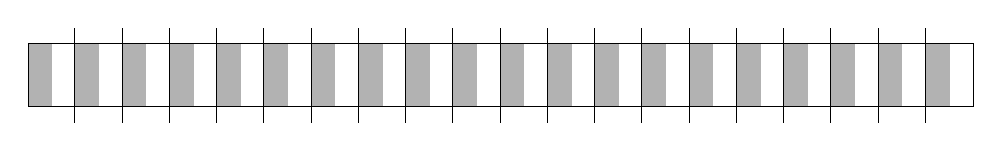
\begin{tikzpicture}
        \foreach \x in {0, 6, ..., 114} {
                \node[inner sep=0, minimum height=8mm, minimum width=3mm, fill=black!30, anchor=south west] at (\x mm, 0) {};
            }
        \foreach \x in {6, 12, ..., 114} {
                \path[draw] (\x mm, -2mm) to ++(0, 12mm);
            }
        \node[inner sep=0, minimum height=8mm, minimum width=120mm, draw, anchor=south west] at (0,0) {};
    \end{tikzpicture}
\end{center}

Jede Kante besteht aus einem trivialen \qq{deterministischen} Eintrag, nämlich dem Index des neuen Knotens, der sich aus dem Kantenindex ableiten lässt, und einem zufälligen Wert (hier weiß).
Wir nehmen nun an, dass jeder Kante~$i$ ein eigener Prozessor~$p_i$ zugeordnet ist.
Kanten aus dem Startgraph kopieren einfach den entsprechenden Wert.
Danach führen alle anderen Prozessoren folgendes Programm parallel aus:

\begin{algorithm}[H]
    $E[2i - 1] \gets$ KnotenId von neuem Knoten\;
    $E[2i] \gets \bot$\;
    \BlankLine
    $s_i \gets $ uniform zufällig aus $\set{1 \ldots 2(i-1)}$\;
    \While{$E[s_i] = \bot$}{
        warte auf nächste Runde\;
    }

    $E[2i] \gets E[s_i]$\;
\end{algorithm}

Dieser Algorithmus funktioniert so gut, weil sich in jeder Runde die erwartete Anzahl an nicht fertiggestellten Kanten halbiert.
Nach der ersten Runde sind alle Kanten fertig, deren $s_i$ ungerade war;
in diesem Fall konnten wir nämlich einfach die \qq{deterministische} Hälfte einer Kante lesen.
Da $s_i$ uniform gezogen wurde, ist $s_i$ mit Wahrscheinlichkeit $1/2$ ungerade.

In der zweiten Runde können wir von den verbleibenden Kanten all jene fertigstellen, die auf eine Kante zeigen, die in der ersten Runde fertig gestellt wurde.
In anderen Worten, solche Kanten haben einen gerades $s_i$, das auf ein ungerades $s_{s_i}$ zeigt --- dies betrifft in Erwartung $1/4$ aller Kanten.

In der $i$-ten Runde setzt sich die Kette analog fort:
Insg. benötigen wir $i-1$ Verweise von gerade auf gerade, gefolgt von einem einzelnen auf ungerade.

Die erwartete Anzahl der Runden der letzten Kante ist also geometrisch mit Erfolgswahrscheinlichkeit $1/2$ verteilt.
In Erwartung sind wir für diese Kante nach $2$ Runden fertig.
Mittels Chernoff-Ungleichung können wir die Wahrscheinlichkeit mehr als $\beta \log n$ Runden zu benötigen für geeignetes~$\beta$ auf $n^{-2}$ beschränken.
Durch union-bound folgt dann, dass der Algorithmus mit hoher Wahrscheinlichkeit eine Laufzeit von $\Oh{\log n}$ hat.

\subsubsection{Abhängigkeiten ausschließen}
Der eben vorgestellte Algorithmus kann auch so abgeändert werden, dass es zu keinerlei expliziten Abhängigkeiten kommt.
Dazu vermeiden wir es einfach vollständig zufällige Vorgänger zu lesen.
Dies ist vor allem im Kontext von verteilten Multicomputern von Vorteil, bei denen Zugriffe auf den Speicher von anderen Computern typischerweise zu erheblicheren Verlangsamung führen.

Die Idee ist simple: statt von einer Position der Kantenliste zu lesen, ziehen wir einfach die Berechnung, die dort stattgefunden haben muss, selbst nach.

Angenommen wir befinden uns an Position~$i$ und ziehen~$s_i$.
Falls $s_i$ ungerade ist, befindet sich dort der Index eines neuen Knotens, den wir einfach nachrechnen können.
Falls $s_i$ gerade ist, müssen wir \qq{nur} denselben zufälligen Vorgänger~$s_{s_i}$ ziehen, der am Index $s_i$ gezogen wurde.

Dieses Oxymoron können wir lösen, indem wir die deterministische Natur unserer Pseudo-Zufallsgeneratoren ausnutzen.
Wir erzeugen an jeder Position der Kantenliste einen Pseudo-Zufallsgenerator, dessen Zustand deterministisch von der Position in der Kantenliste abgeleitet werden kann.
Man könnte beispielsweise einfach den Index als Seedwert für den Generator nutzen.

Hierbei müssen wir allerdings vorsichtig sein, da Pseudo-Zufallsgeneratoren in der Regel eine sogenannte Burn-in Phase benötigen, da die ersten Werte ungewünschte Eigenschaften besitzen können.
Außerdem ist das Erzeugen eines Zufallszahlengenerators oft sehr viel teurer als das Ziehen eines Zufallswortes.
Daher nutzen die Autoren~\cite{SANDERS2016489} statt eines dedizierten Pseudo-Zufallsgenerator eine zufällige Hashfunktion.

Dies ist eine pragmatische Entscheidung und liefert --je nach Hashfunktion-- eine vergleichsweise kleines Ensemble an möglichen Ausgaben.
Empirisch scheinen aber die erzeugten Graphen ähnlich zu BA Graphen zu sein.
Daher kann der Generator ---gerade bei verteilten Berechnungen--- das Mittel der Wahl sein.

\subsection{Skalenfreie Netze}
Skalenfreie Netz (scale-free network) sind Graphen mit Power Law Gradverteilungen (Gegendarstellung: \cite{doi:10.1073/pnas.200327197});
hierbei handelt es sich um einen sehr gebräuchlichen Begriff in der Network Science Literatur.
Der Begriff selbst hat zwei (verwandte) Erklärungen, die uns noch ein Einblicke in die Eigenschaften von Power Law Verteilungen erlauben.

\subsubsection{Skaleninvariant}\label{subsec:scaleinvariant}
Wir können \qq{skalenfrei} als \qq{skaleninvariant} auffassen.
Damit wird auf die Selbstähnlichkeit der Power-Law Verteilung hingewiesen:
eine perfekte Power Law Verteilung ist in einem Log-Log-Plot immer eine Grade mit Steigung $-\gamma$.
Dabei ist unerheblich wie groß der zugrunde liegende Objekt (hier Knotenmenge) ist.

Wir können also die Verteilung umskalieren, \zB die Knotenanzahl um einen Faktor $a$ vergrößern.
Dann gilt für die entsprechende Zufallsvariablen $X$ und $X'$:

\begin{align}
    \prob{X = k}   &                                                                                           & \propto k^{-\gamma}  \label{eq:prop-scalefree-1} \\
    \prob{X' = ak} & \propto (ak)^{-\gamma} = \underbrace{a^{-\gamma}}_{\text{unabhängig von $k$}} k^{-\gamma} & \propto k^{-\gamma}\label{eq:prop-scalefree-2}
\end{align}

Beobachte, dass die Proportionalität in \cref{eq:prop-scalefree-1,eq:prop-scalefree-2} jeweils andere Normierungen verbirgt.

\subsubsection{Unbegrenztes Wachstum}
Der Begriff \qq{scale-free network} wird regelmäßig Barab{\'{a}}si und Albert, den Autoren des BA Modells, zugeschrieben.
Barab{\'{a}}si selbst erklärt den Begriff über das unbeschränkte Wachstum des $k$-ten Moments der Power Law Verteilung für $n \to \infty$.

Das $k$-te Moment einer kontinuierlichen (Grad)Verteilung $p(d)$ ist definiert als:
\begin{align}
    \langle d^k \rangle = \expv{X^k} = \int_\dmin^\dmax d^k p(d) \intd d,
\end{align}
wobei $X \follows p$ eine nach $p$-verteilte Zufallsvariable ist.

Für $k=1$ erhalten wir also den Erwartungswert, $\langle d^2 \rangle$ ist essentiell in der Berechnung der Varianz $\langle d^2 \rangle - \langle d \rangle^2$, $\langle d^3 \rangle$ beeinflusst die Schiefe (skewness) et cetera.
Bezogen auf Power Law Verteilungen ergibt sich:
\begin{align}
    \langle d^k \rangle
     & = \int_\dmin^\dmax d^k C d^{-\gamma} \intd d
    = C \left[ \frac{1}{k + 1 - \gamma} d^{k + 1 -\gamma}\right]_\dmin^\dmax    \\
     & = C \frac{\dmax^{k + 1 -\gamma} - \dmin^{k + 1 -\gamma}}{k + 1 - \gamma}
\end{align}

Das Verhalten des $k$-ten Moments für $n \to \infty$ (und dadurch $\dmax \to \infty$) wird also maßgeblich durch $k + 1 - \gamma$ beschrieben:
\begin{itemize}
    \item Für $k + 1 < \gamma$ konvergiert $\lim_{\dmax \to \infty} \dmax^{k + 1 -\gamma} = 0$.
          Somit ist $\langle d^k \rangle$ endlich.

    \item Für $k + 1 = \gamma$ ist das $k$-te Moment konstant.

    \item Für $k + 1 > \gamma$ divergiert das $k$-te Moment und wächst grenzenlos.
\end{itemize}

\noindent
Bisher nahmen wir $2 < \gamma \le 3$ an.
In diesem Regime konvergiert $\langle d \rangle$, somit erwarten wir, dass der Durchschnittsgrad in einem wachsenden Netz irgendwann stagniert.
Dies widerspricht aber scheinbar unserer Analyse in \cref{subsec:groesse_von_hubs}, wo wir zeigten, dass der Grad von Hubs polynomiell in der Knotenanzahl wächst.
Dem wird aber schlicht dadurch Rechnung getragen, dass die Varianz über das divergierende zweite Moment $\langle d^2 \rangle$ wächst.
Polemisch gesagt, werden also Hubs als Outlayer verbucht.
Ein zufällig gezogener Knoten kann kleinen oder großen Grad haben mit einem Streuung über viele Größenordnungen --- es gibt also kein Konzept von Größenverhältnissen (engl., scale).